\lstset{style=c_sharp}
  %----------------------------------------------------------------------------
\chapter{Felhasznált technológiák}


A Cronotus alkalmazás két jól elkülöníthető részre bontható fel. Amint a \ref{fig:architecture_overview}-es ábrán is látható, a felhasználói felület weben keresztül érhető el, mely a React\cite{reactdocs} technológia segítségével lett megalkotva TypeScript\cite{typescriptdocs} nyelven, míg az alkalmazás szerver oldali része egy .NET keretrendszeren\cite{dotnetnocs} alapuló program, mely C\# nyelven\cite{csharpdocs} lett megírva és az Entity Framework Core\cite{entityframeworkdocs} által lefektetett szabályrendszert használva kommunikál egy Microsoft SQL Server\cite{sqlserverdocs} adatbázissal, ahol minden adat eltárolásra kerül.
Ahhoz, hogy ezeket az adatokat a felhasználó elérhesse, a kliens és szerver oldal között egy REST API\cite{restfuldocs} segítségével történik meg a kommunikáció.

\begin{figure}[h]
    \centering
    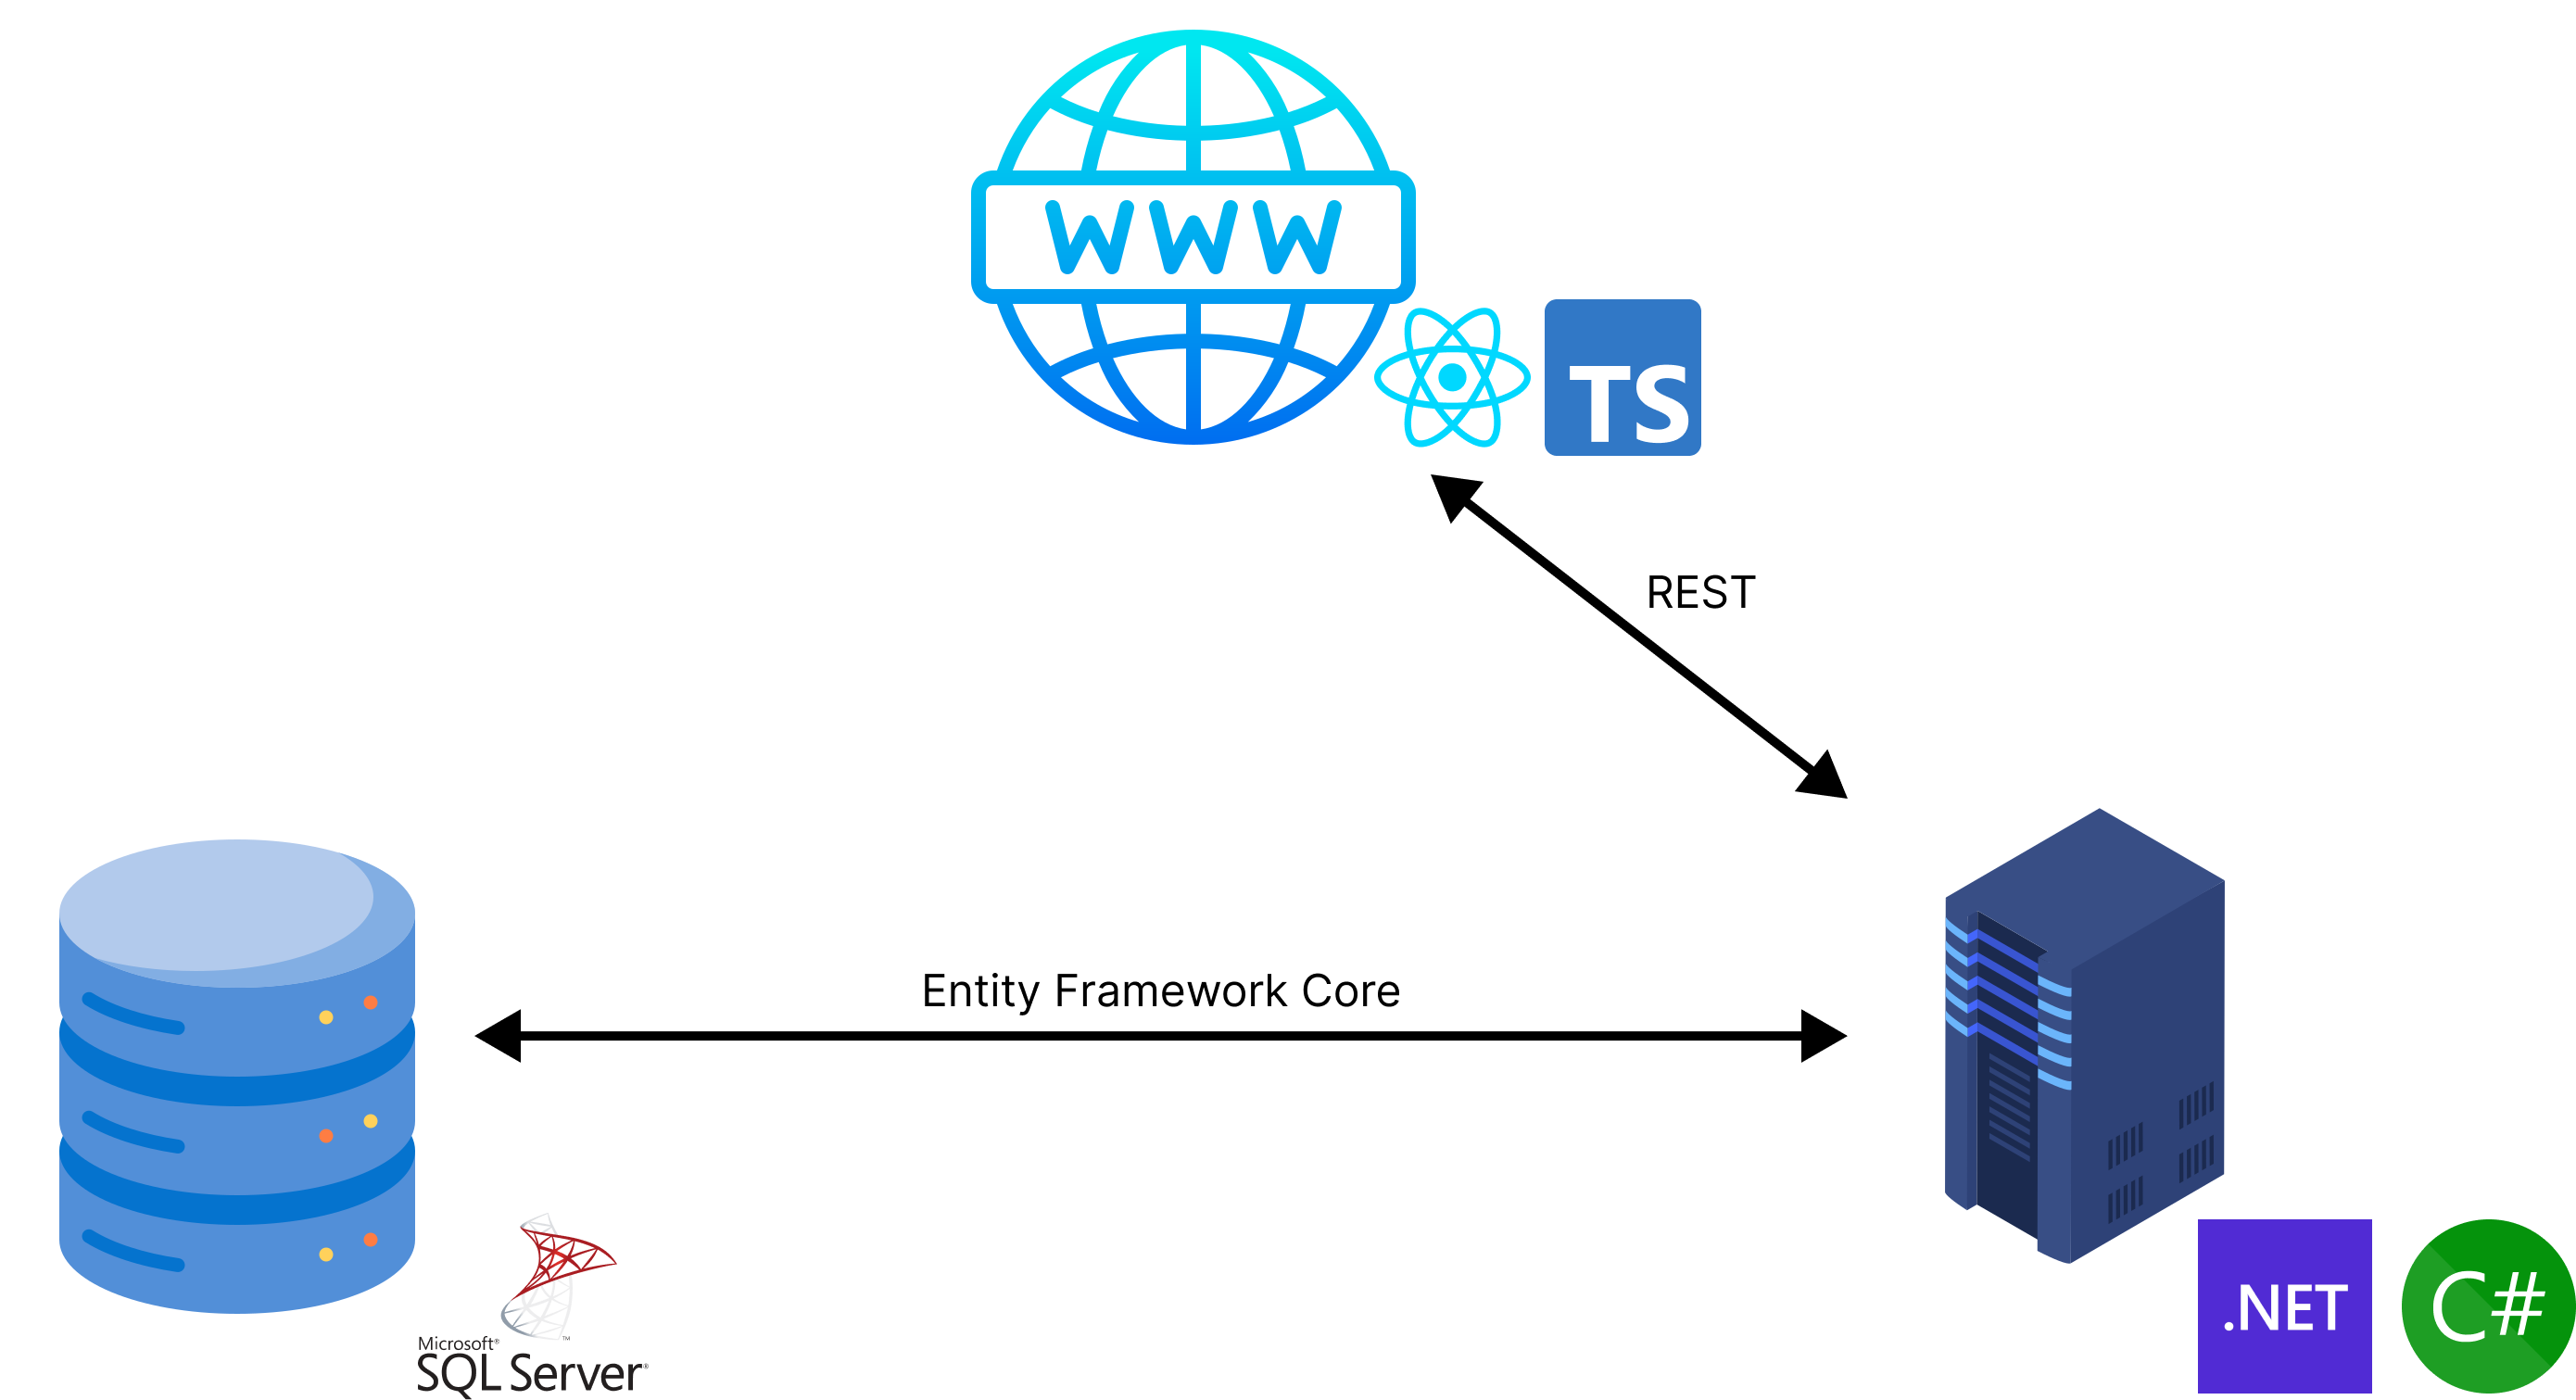
\includegraphics[width=0.8\textwidth]{./images/cronotus_architecture_overview.png}
    \caption{Rendszer architektúra komponensekre bontva}
    \label{fig:architecture_overview}
\end{figure}

%----------------------------------------------------------------------------

%----------------------------------------------------------------------------
\section{A szerver}

A szerver feladata az, hogy kiszolgálja a webalkalmazásról beérkező kéréseket. Ez a feladat alapszinten viszonylag könnyen elvégezhető lenne, viszont nem elég csak csupán elvégezni, hanem a legmegfelelőbb módon kell ezt véghez vinni. Fontos szem előtt tartani a biztonságot, kérésenkénti időt, illetve megbízhatóságot. Az első fontos döntés a szerverrel kapcsolatban az, hogy milyen architekturát valósít meg. A Cronotus esetében egy rétegelt architekturáról\cite{onionarchitecturedocs} beszélhetünk, mely három fő elemre bontja a szerver működését.

\begin{figure}[h]
    \centering
    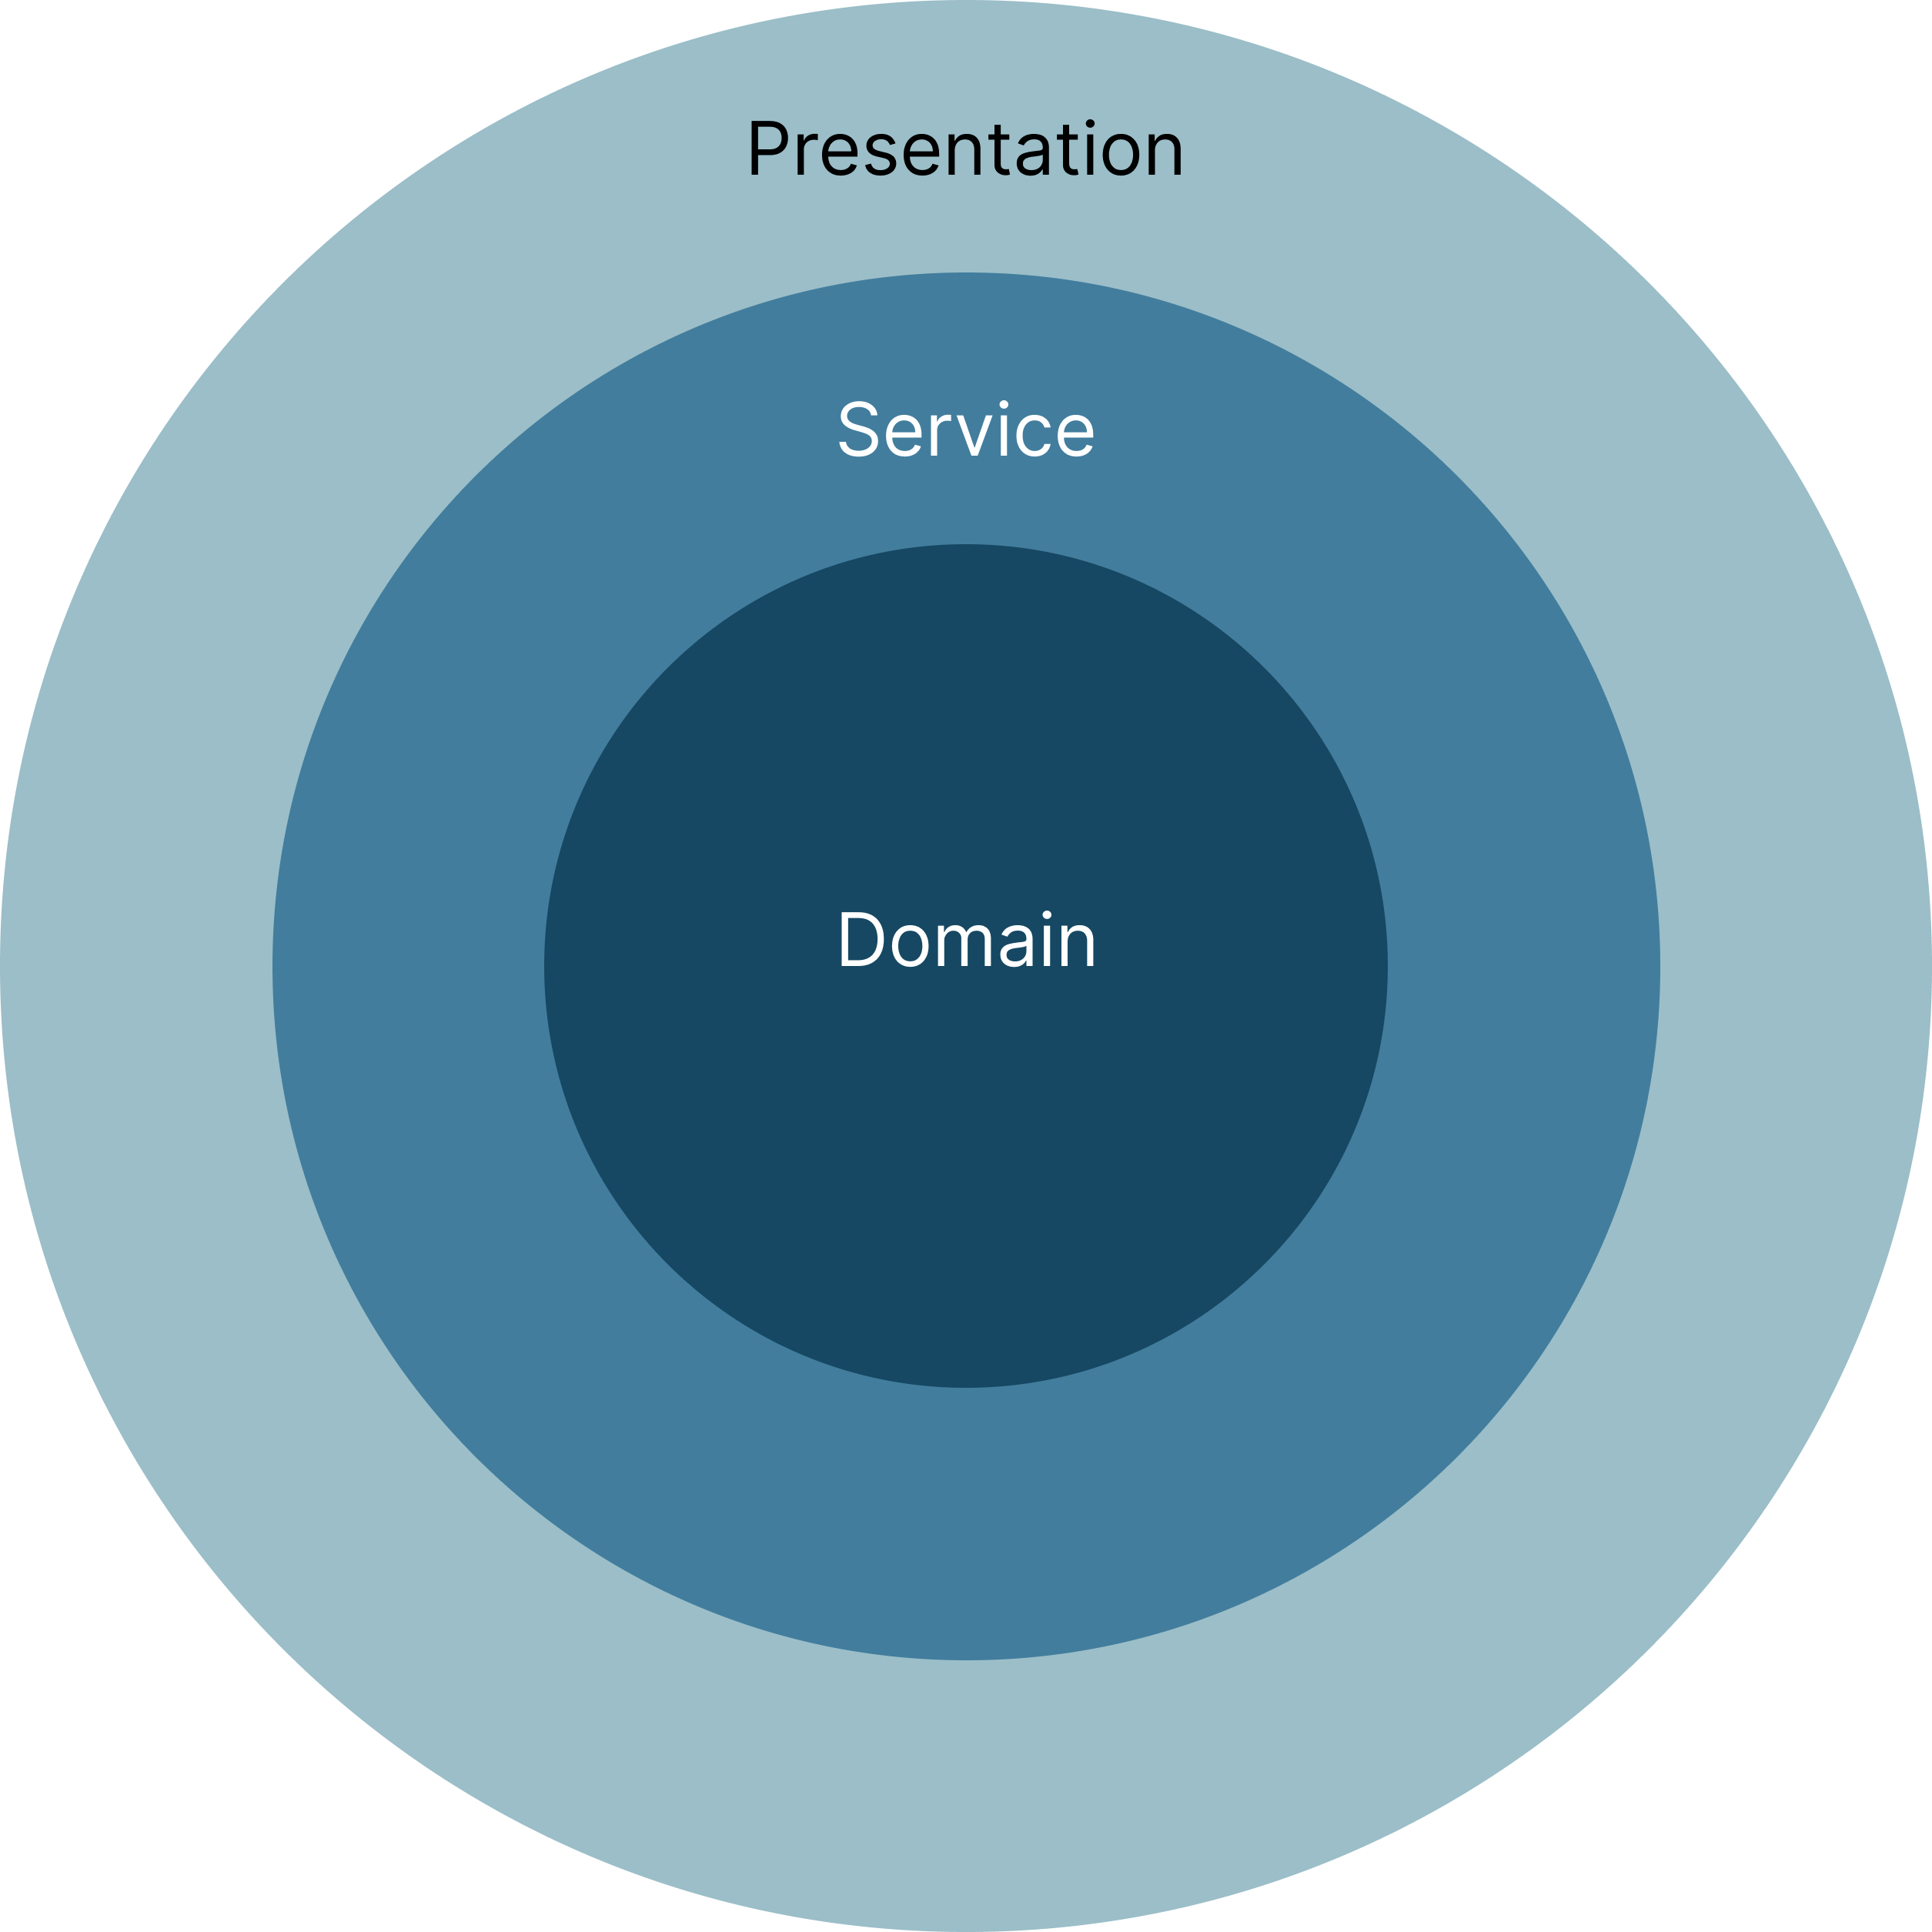
\includegraphics[width=0.6\textwidth]{./images/backend_onion_architecture.png}
    \caption{A rétegelt szerver architektúrája}
    \label{fig:server_onion_architecture}
\end{figure}

A három réteg a \ref{fig:server_onion_architecture}-es ábrán feltüntetett módon helyezkedik el. A legalsó szint a Domain, melynek mindössze annyi a feladata, hogy az adatbázissal kommunikáljon. Ezen a szinten történik meg az adatok kinyerése, vagy akár az alapszintű műveletek véghezvitele, például létrehozás, vagy törlés.

A kör középpontjától kifele haladva a következő a Service réteg. Ez az a szint, amely a biznisz logikát végrehajta a kapott adatokon. Abban az esetben, ha a kliens oldal egy kérést küld valameny adat lekérésére, úgy a kéréshez szükséges eredmény ezen a szinten formálódik olyan alakba, amely megfelelő a fogyasztónak. A szint felelősége úgy is felfogható, mint egy tolmács, mely a kliens és Domain között működik. Főbb feladatai a komplex struktúrájú adatok egyszerű alakra és utasításokra bontása, illetve egyszerű adatok előkészítése és prezentálható formába szervezése a kliens számára.

A legfelső, a Presentation réteg feladata a fogyasztó irányába történő kérésekkel kapcsolatos visszajelzések megfelelő kezelése, illetve a Service rétegtől kapott adatok átirányítása a helyes HTTP kóddal.

\subsection{A rétegelt architektúra előnyei}

Felmerülhet a kérdés, hogy miért érdemes az előbbiekben [\ref{fig:server_onion_architecture}] bemutatott formába szervezni a szerver felépítését. 
Ahhoz, hogy ezt bemutassuk, fontos először megvizsgálni az architektúrán belüli egyes rétegek közti függőségek folyását. 
Ha ezt a felépítést követjük, akkor a függőségek a legbelső szintektől a felsőbb szintek irányába folynak, azaz a Domain réteg nem függ semmítől. 
Ez betudható szabályként is, tehát egy réteg minél alacsonyabban van a felépítésben, annál kevesebb függősége van.
Az előbbiekben leírt függőségi irányzat úgy is nevezhető, mint az úgynevezett Inversion of Control (IoC) \cite{inversionofcontroldocs}.

Továbbá minden réteg csakis kizárólag az alatta levő rétegre hivatkozhat. Ez azért hasznos, mert így nem kall aggódnunk afelől, hogy hogyan fog egy felsőbb szintű művelet implementálni egy alacsonyabb osztályút, elég kontraktokat felállítanunk, melyeket teljesíthetnek a felső rétegek. Ez fontos tulajdonsága az architektúrának, hiszen nagy szabadságot nyújt egyes szintek elkészítésében, hiszen elég csak az oda tartozó logikára figyelnünk.

\begin{figure}[h]
    \centering
    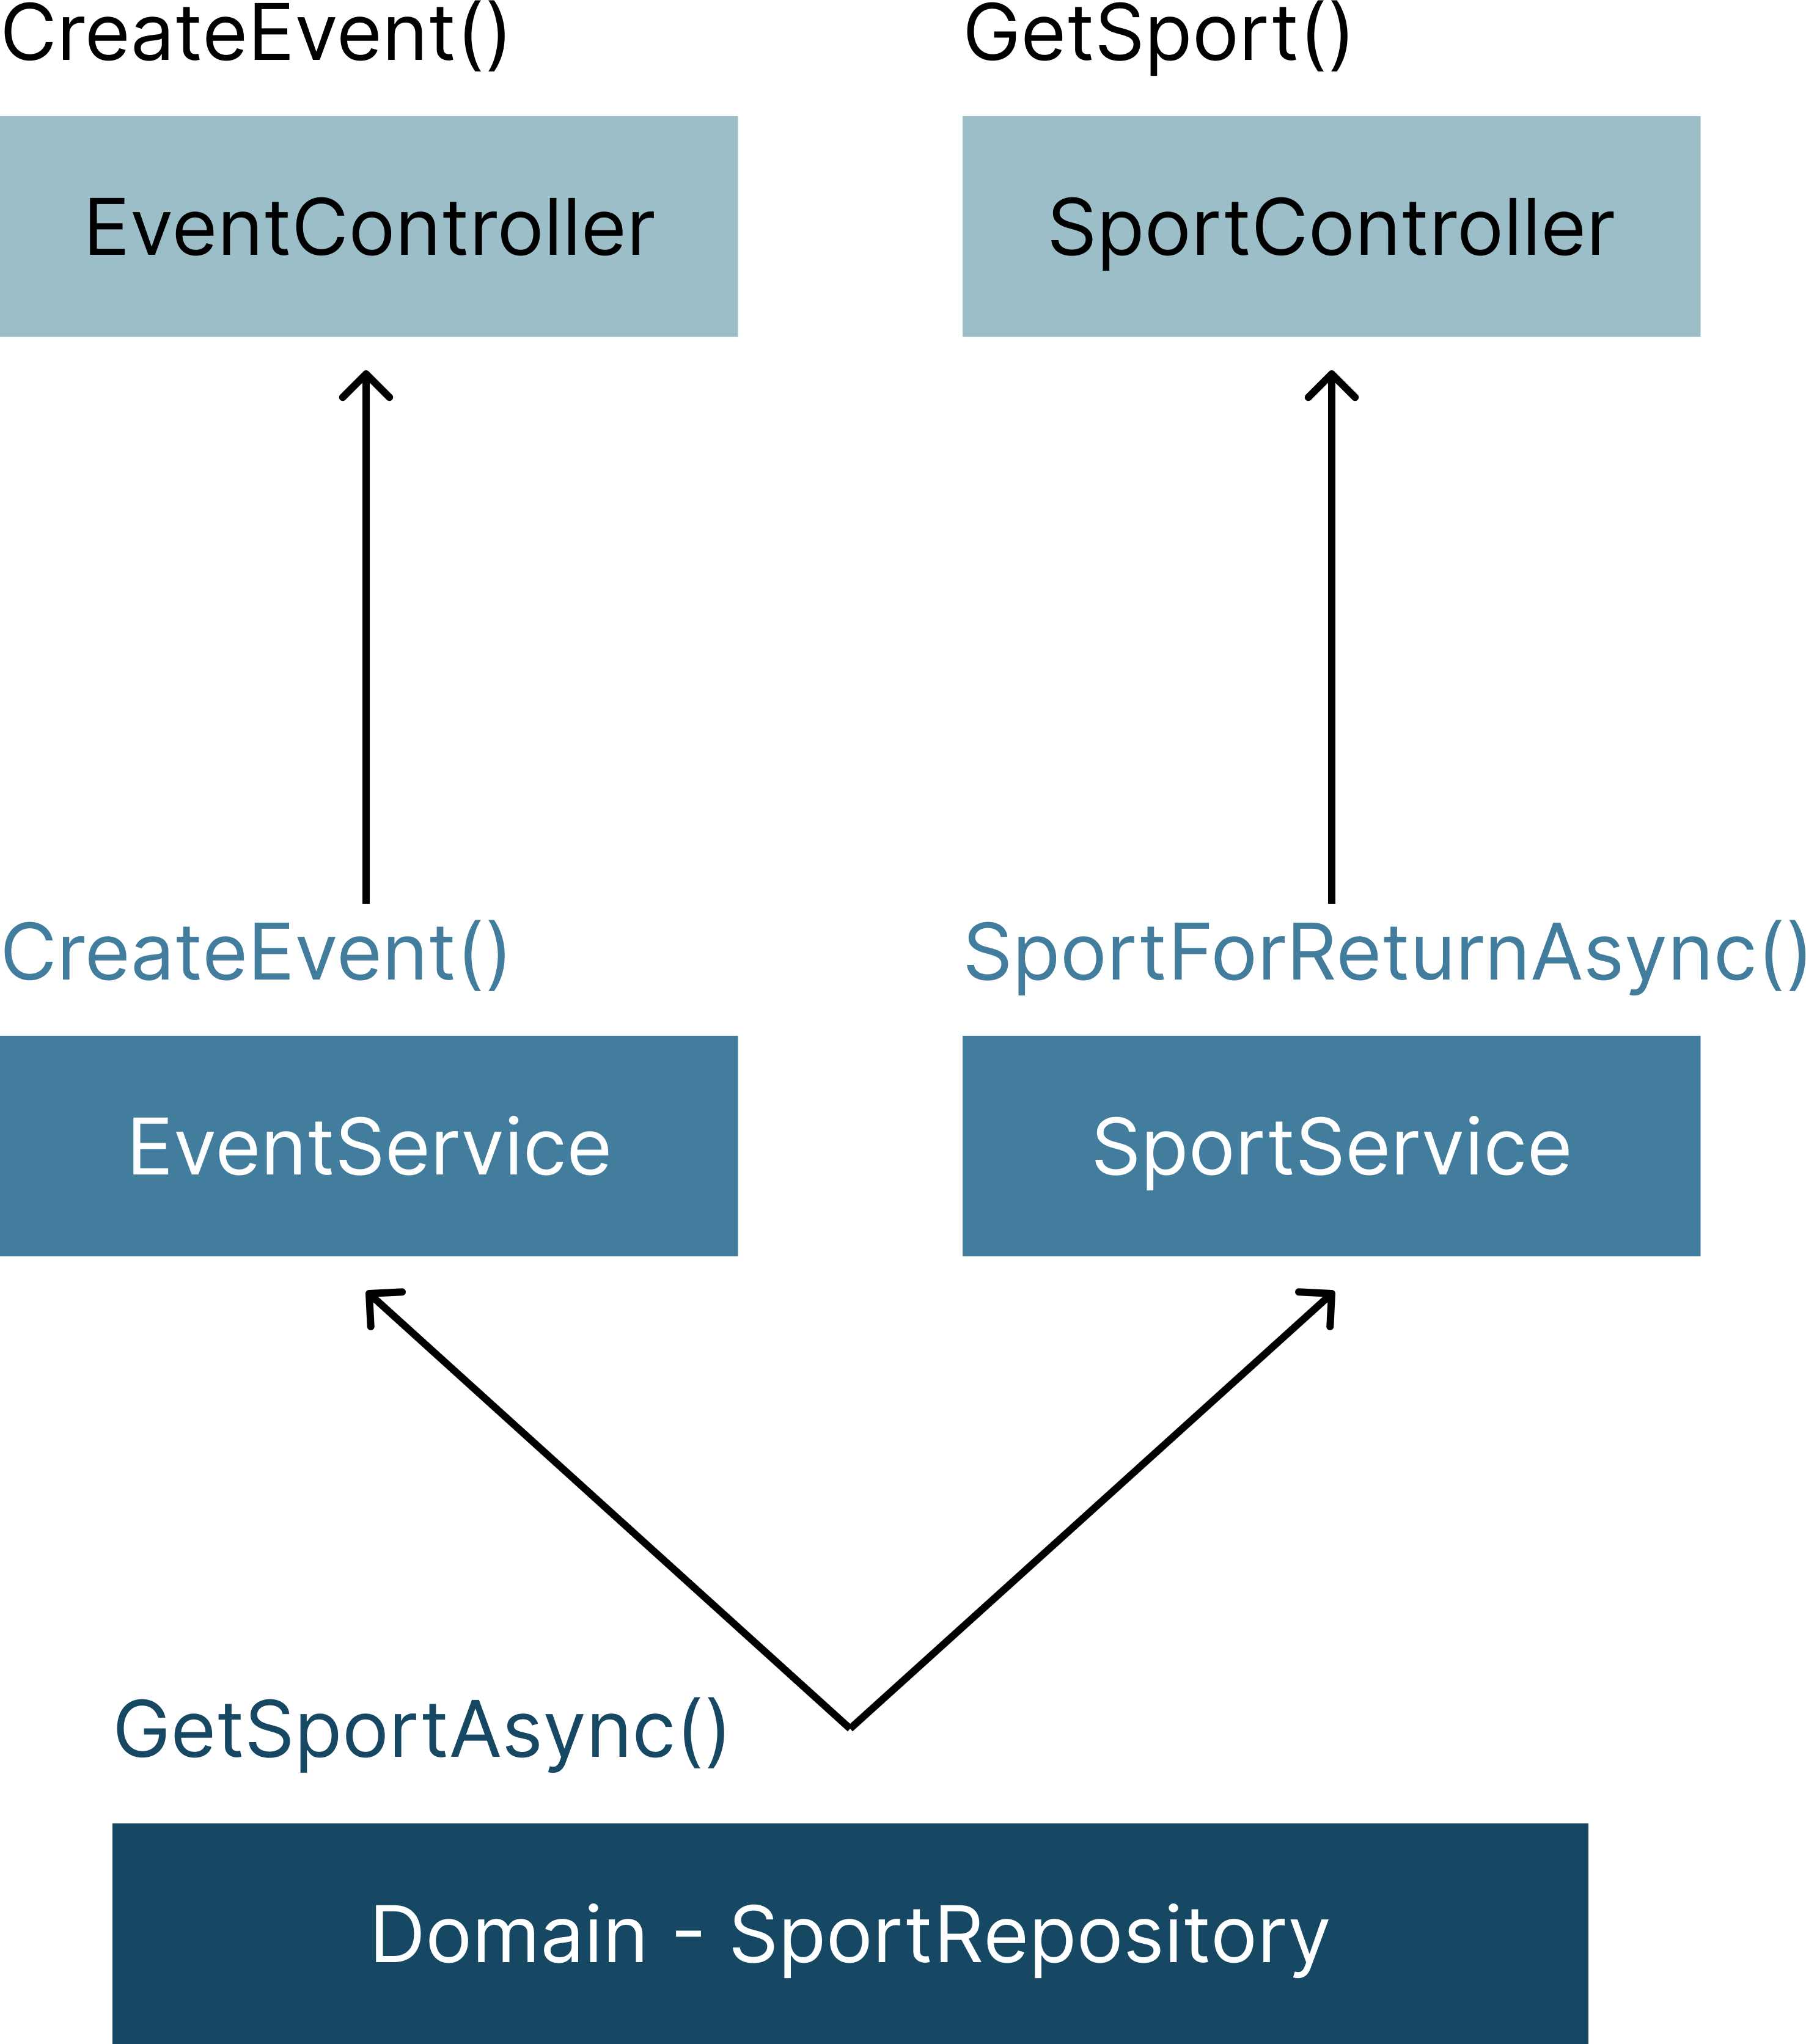
\includegraphics[width=0.6\textwidth]{./images/get_sport_example.png}
    \caption{A SportRepository egy Domain szintű műveletének eredményének kétféleképpen való felhasználása felsőbb szinteken}
    \label{fig:sport_repo_usage_example}
\end{figure}

A \ref{fig:sport_repo_usage_example}-as ábrán látható egy példa, mely a rétegelt architektúra egy előnyét használja fel. A SportRepository-ban rendelkezésünkre áll egy függvény, mely egy Sport Entity-t térít vissza. A Repository-nak ebben az esetben nem kell tudnia, hogy hogyan fogják a felsőbbrendű rétegek felhasználni az innen kapott adatot. Az EventService arra használja fel az adatot, hogy ellenőrzés alá vesse a létrehozandó eseményhez kiválasztott sportot, vajon létezik-e? A SportService viszont arra használja fel ugyanazt az eredményt, hogy egy prezentálható formában vissza térítse a Presentation szintnek a sportot, ami egy Controller formájában elérhetővé teszi a kliens számára, hogy lekérhessen egy sportot ID alapján.

\subsection{Az adatbázis}

A rendszer adatai egy Microsoft SQL Server relációs adatbázisban\cite{relationaldatabasedocs} vannak eltárolva. Mivel a rendszer személyes információkat tárol el a felhasználóiról, szükséges volt egy olyan adatbázist választani, mely megfelelő képpen tudja kezelni az egyes felhasználók és felhasználókhoz kötődő entitások közötti kapcsolatokat. Továbbá az is fontos, hogy biztonságosan legyenek az adatok tárolva. Mindezeket  figyelembe véve egy relációs adatbázis volt a legjobb választás. A konkrét döntés azért esett a Microsoft SQL Server termékre, mivel a szerver fő keretrendszere alapból Microsoft termék, így a Microsoft-készített adatbázis egy jó integrálhatósági lehetőségnek bizonyul. Továbbá a technológiák megegyezése elősegít a későbbi felhőbe való kitelpítésben is.

Az adatbázis strukturális létrehozása a \textit{code first approach}\cite{codefirstapproachdocs} elv segítségével hajtódik végre, ahogyan a \ref{fig:code_first_approach}-es ábrán is látható. Az Entity Framework Core lehetővé teszi azt, hogy adatmodellek és adatmodellek közti kapcsolatok alapján migrációk segítségével változtassunk az adatbázis sémán, illetve az abba tartozó adatokon.

\begin{figure}[h]
    \centering
    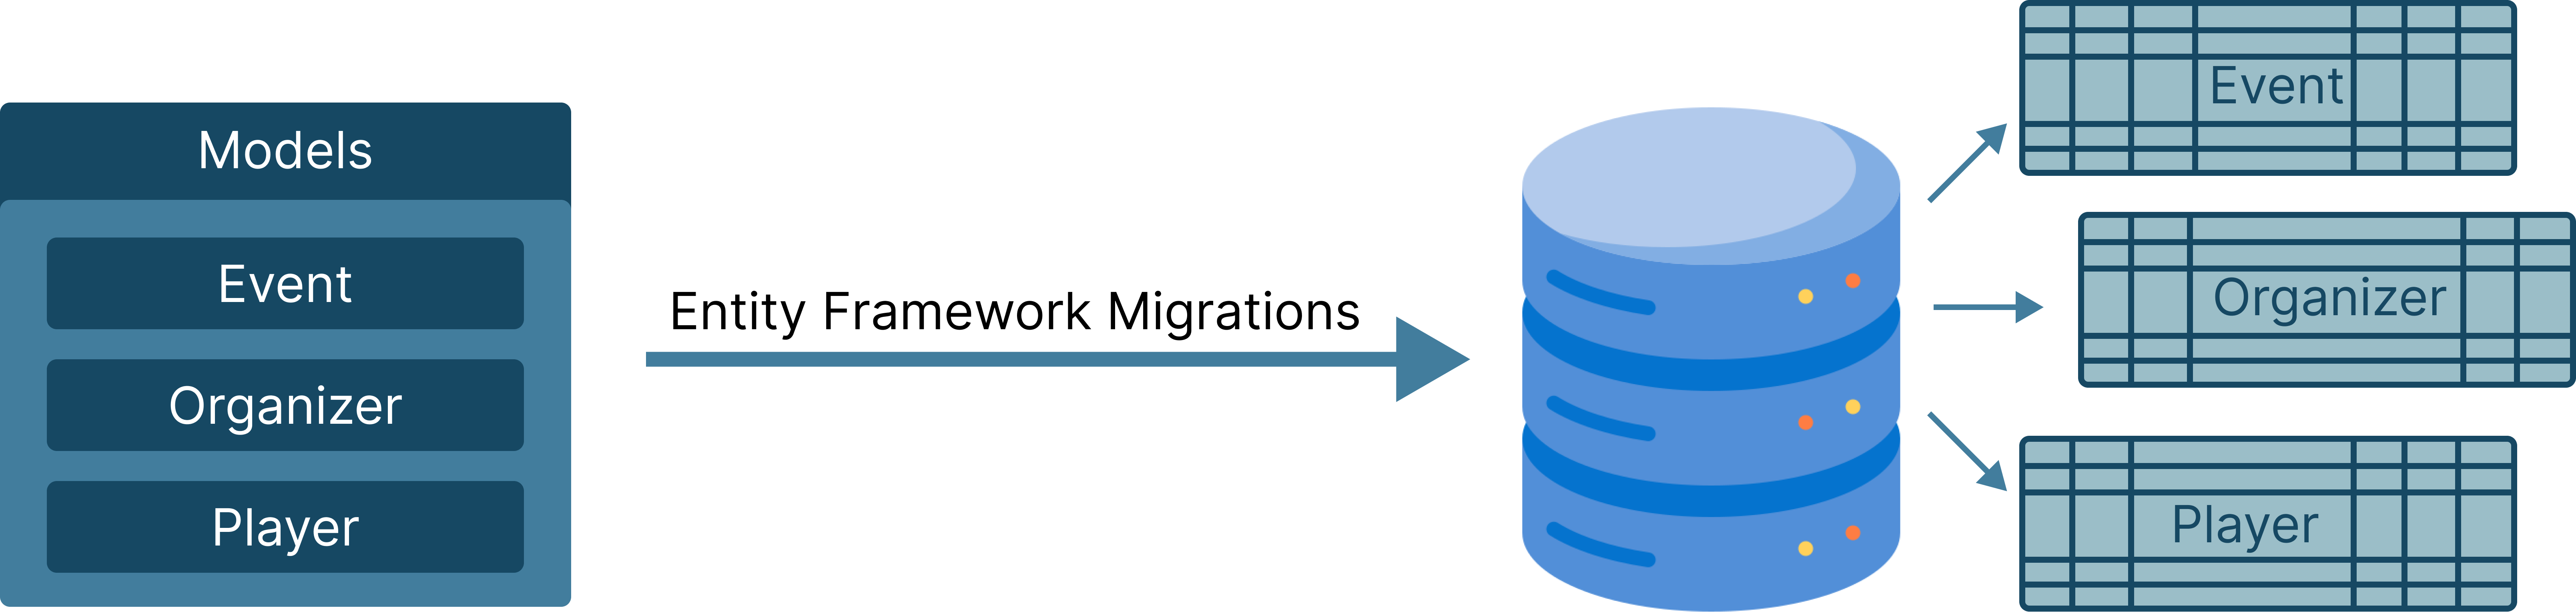
\includegraphics[width=\textwidth]{./images/code_first_approach.png}
    \caption{A Code First Approach áttekintése}
    \label{fig:code_first_approach}
\end{figure}

Technikailag megvizsgálva, a Code First Approach [\ref{fig:code_first_approach}-es ábra] az Entity Framework Core egyik hozománya, mely az ORM (Object Relational Mapper)\cite{codefirstapproachdocs} segítségével képes a \textit{DbContext} osztályon keresztül kapcsolatba lépni az adatbázissal, továbbá a \textit{RepositoryBase} absztrakt osztályon végrehatjtandó CRUD műveletek\cite{crudoperationdocs} segítségével tudja az itt tárolt entitásokat kezelni, törölni vagy újakat létrehozni.

\subsection{A Cronotus API}

A kliens oldali kéréseket a szerver a Presentation [\ref{fig:architecture_overview}-es ábra] rétege fogadja és szolgálja ki. A \textit{pipeline}-ja HTTPS (HyperText Transfer Protocol Secure)\cite{httpsdocs} protokolt követve üzemel. A kliens HTTP kéréseket küldve tud adatokat küldeni, lekérni, illetve szerveri erőforrásokat igénybe venni adatokkal kapcsolatos műveletekhez. Az adatokat DTO-k (Data Transfer Object)\cite{dtodocsmicrosoft} formájában cserélgeti a kliens a szerver oldallal, mely JSON (JavaScript Object Notation)\cite{jsondocs} formájában valósul meg. 

A szerver minden beérkező kérést átfuttat egy ellenőrzésrendszeren [\ref{fig:pipeline}-ös ábra], mely az Application Pipeline formájában van felépítve. Itt biztonsági és adatintegritási szempontból fontos vizsgálat alá veti a kéréseket. A szerver a pipeline-ban érvényesíti azt, hogy HTTP helyett biztosan HTTPS protokllon keresztül történjen meg a kommunikáció, hiszen így egy harmadik fél nem tudja leolvasni a küldött kérések tartalmát, úgy sem ha hozzáférése van ezekhez, mivel kódolva vannak. A pipeline továbbá más hasznos beállításokat is érvényesít, például azt, hogy csak megfelelő URL címekről legyen engedélyezett a hozzáférés a szerverhez, illetve jogosultságot vizsgál \textit{Authentication} és \textit{Authorization}\cite{authflowsdocs} segítségével.

\begin{figure}[h]
    \centering
    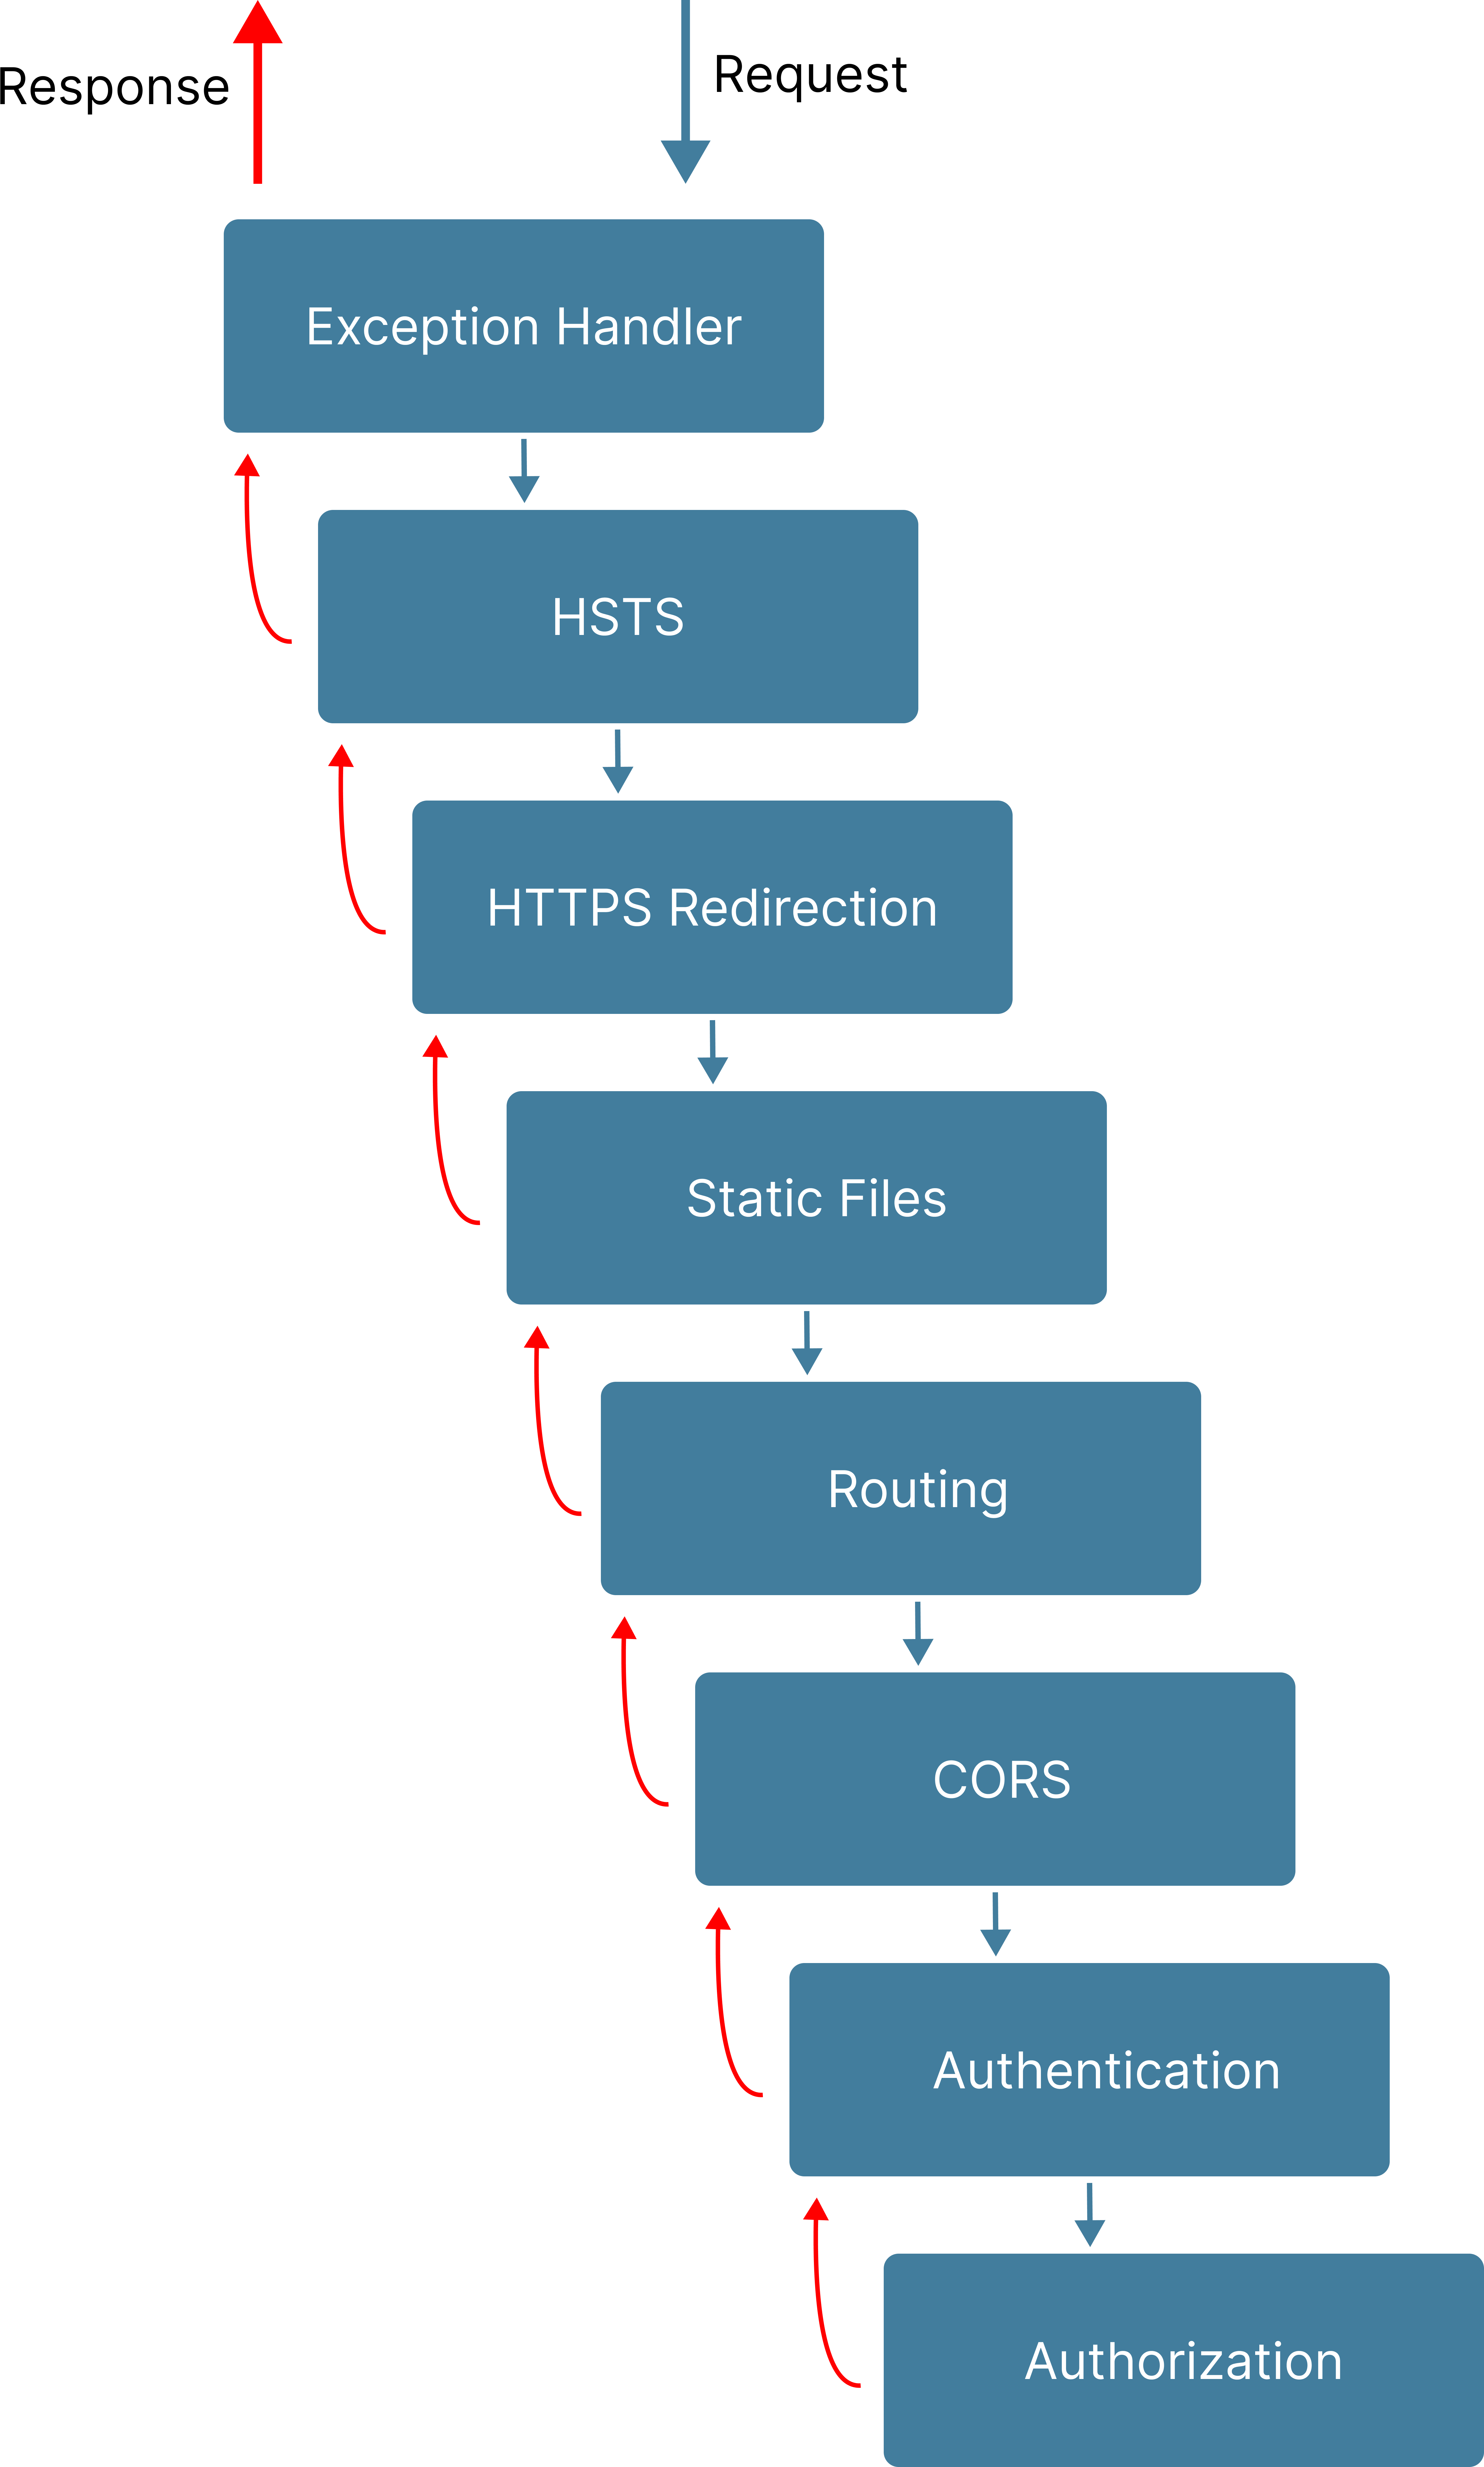
\includegraphics[width=0.6\textwidth]{./images/pipeline.png}
    \caption{A pipeline, melyen keresztül kell mennie minden szerver fele érkező kérésnek}
    \label{fig:pipeline}
\end{figure}

\subsection{Hitelesítés és Engedélyezés}

Az rendszer JWT Tokenek\cite{jwtdocs} formájában kezeli a felhasználói munkamenetet és az ezekbe kódolt információk segítségével végzi el a felhasználók hitelesítését és bírálja el az \textit{endpoint}-okhoz való hozzáférésüket.

Egy ilyen token fontos információkat tartalmaz, például felhasználói jogok, jogokhoz kapcsolódó id-k, illetve a token lejárati dátuma. 

A kliens oldalról kapott kérések mindegyikéhez csatolva van egy ilyen JWT token, amit a rendszer egy kérés beérkeztekor dekódol, majd az innen kinyert információk segítségével megnézi, hogy érvényes-e a token, majd ellenőrzi, hogy a felhasználónak van-e joga végrehajtani a kívánt műveletet. Egy token élettartama 10 perc, ezután egy \textit{Refresh Token} segítségével a kliens újat kell kérjen. Ez a fajta viszonylag rövid szsavatossági idő egy fontos biztonsági intézkedés, mivel ha egy harmadik fél meg is tud szerezni egy ilyen érvényes tokent, akkor is csak maximum 10 perce van arra, hogy hozzáférése legyen a szerverhez. 

\subsection{Globális hibakezelés}

Annak érdekében, hogy a kód átlátható és könnyen karbantartható legyen a hiba és kivételkezelést a projekt egy globális hibakezelő middlware segítéségvel oldja meg, mely részét képezi az application pipeline-nak.

Ha ezt a kezelési módszert használjuk, akkor nincs szükség \textit{try - catch} kódblokkok használatára, hiszen ha valamilyen kivétel merül fel, akkor azt elég csak tovább dobni, majd a middleware automatikusan lekezeli. A kezelés során a middleware beállítja a visszatérítendő objektumba a fellépő hiba HTTP státuszkódját, majd a kiindulási pontból dobott hiba üzenetét, mindezt annak érdekében, hogy kliens oldalon könnyen olvasható legyen, hogy egyes hiba miből származhat.

%----------------------------------------------------------------------------
%----------------------------------------------------------------------------
\section{A felhasználói felület}

A felhasználói felület egy webalkalmazás formájában nyilvánul meg. A felhasználók itt végezhetnek eseményekkel kapcsolatos műveleteket, például létrehozás, csatlakozás, vagy kommentelés. Ez az alfejezet a felhasználói felület felépítését és működését tárgyalja.

\subsection{Felhasznált technológia}

A webalkalmazás TypeScript\cite{typescriptdocs} nyelven íródott, React\cite{reactdocs} könyvtár felhasználásával.
A TypesScript a JavaScript\cite{javascriptdocsmozilla} nyelvet bővíti ki egy szintaxis csomaggal, amely lehetővé teszi a változók és objektumok típuskezelését, ezzel egy jobban átlátható és biztonságosabb fejlesztési procedúrát nyújtva.

A React könyvtár segítségével a webalkalmazás egy Single Page Application (SPA)-ként\cite{singlepageapplicationdocs} működik.
A SPA az egész weboldalt egyetlen HTML dokumentumban építi fel, majd változás során ennek a tartalmát frissíti és cseréli. Ez előnyös megoldás, mivel így nem kell minden oldalcsere, illetve tartalomfrissítés után újratölteni az alkalmazást, így gyorsabb lesz, javítja a felhasználói élményt.

Az alkalmazáshoz felhasznált további könyvtárcsomagok kezelése, a webalkalmazás futtatása, illetve építése a Vite\cite{vitedocs} segítségével van megoldva.
A Vite egy gyors és egyszerű build eszköz, mely alkalmas React webalkalmazások kezelésére. Lehetővé tesz Live Reloading-ot mely hasznos a fejlesztés során, illetve úgy van felépítve, hogy minimalizálja az alkalmazás építéséhez szükséges időt, így mégjobban gyorsítva és javítva a fejlesztési időt, élményt.

Az alkalmazás felhasználói felületének egy szerves része továbbá a React könyvtárra épített Material UI komponens csomag, mely segítségével könnyen és gyorsan lehet előre megépített megjelenítő komponenseket felhasználni.

\subsection{Kommunikáció a szerverrel}

A webalkalmazás HTTPS protokollon keresztül kommunikál a szerverrel. A HTTPS protokoll a HTTP protokoll biztonságos formája. Itt a HTTP-vel ellentétben az adatok nem egyszerű szöveges formátumban vannak küldve, hanem kódolt blokkokként, melyek biztosítják azt, hogy út közben egy rosszindulatú harmadik félnek ne legyen hozzáférése bármilyen kommunikációhoz.

Az alkalmazás GET metódusokra az SWR - Data Fetching\cite{swrdocs} könyvtárcsomagot használja. Az SWR rövidítés az angol ``stale-while-revaildate'' szókapcsolatoban ered, mely annyit tesz, hogy ``elavult-közben-újraérvényesít''. Az SWR adatlekérési stratégia alapján egy kérés után előszőr a potenciális elavult adatot megkapjuk egy cache (stale) tároló rendszerből, majd elküldjük a kérést a legfrissebb adatért (revalidate), majd végül előállunk ezzel.

A könyvtárcsomag lehetőséget biztosít arra is, hogy az adatlekéréssel kapcsolatos státuszokat kezeljük, például kérés alatt töltés ideje, illetve hibákat. Ezt egyszerűen megtehetjük a függvényhívás esetén, amint a \ref{lst:typescript_example}-es kódrészleten is látszik.

\begin{lstlisting}[caption={SWR használata profil adatok lekérésére}, label={lst:typescript_example}]
const { data: profileInfo, isLoading, error, mutate } = useProfile(userId!);

{isLoading ? (
            <ProfileTitleIsLoading />
          ) : (
            <ProfileHead
              profileInformation={profileInfo!}
              className="profile-head"
            />
          )}
\end{lstlisting}

A \ref{lst:typescript_example}-es ábrán látható, hogy abban az esetben, ha az adatok még lekérés alatt vannak, a komponens a ``ProfileTitleIsLoading'' komponenset tölti be, majd amint a a betöltés befejeződik, megjeleníti a betöltött adatokat.

Amennyiben a szerverhez intézett HTTP kérés nem GET metódus, úgy az alkalmazás nem SWR-t használ, hanem egy egyszrű, dinamikusan felépített fetchert. Ez a fetcher függvény újrahasznosítható, így elég minden egyedi kérés esetében csak megadni a megfelelő adatokat, endpoint címet, és meghívni az ehhez tartozó fetchert.

A \ref{fig:fetchingData}-os ábra szemlélteti néhány végpont egyszerűsített működését.

\begin{figure}[ht]
  \centering
  \includegraphics[width=\textwidth]{./images/fetchingData.png}
  \caption{Néhány endpoint működése}
  \label{fig:fetchingData}
\end{figure}

\subsection{Oldalak közötti navigálás}

A webalkalmazáson való oldalak közötti navigációért a React Router\cite{reactrouterdocs} könyvtárcsomag felelős. Ez lehetővé teszi azt, hogy könnyen és zökkenőmentesen tudjunk oldalak között navigálni, illetve ennek során információt cserélni egyes oldalak, komponensek között.

A React Router lehetővé teszi azt, hogy deklaráljunk minden létező oldalt egy ``Router'' komponensben, ahonnan aztán a Single Page Application dinamikusan cserélni tudja a pillanatynyilag megjelenített oldalt. Ez a deklarálási módszer látható a \ref{lst:router_component}-as kódrészletben.

\begin{lstlisting}[caption={Route-ok deklarálása}, label={lst:router_component}]
const Router = (props: { onLogout: () => void }) => {
  return (
    <Routes>
      <Route path="/" element={<Layout />}>
        <Route index element={<Home />} />
        <Route path="browser" element={<Browser />} />
        <Route path="create-event" element={<CreateEvent />} />
        <Route path="event/:id" element={<SportsEvent />} />
        <Route path="profile" element={<Profile onLogout={props.onLogout} />} />
        <Route path="*" element={<NoMatch />} />
      </Route>
    </Routes>
  );
};
\end{lstlisting}

Abban az esetben, ha kliens oldalon böngészőn belül nem a megfelelő cím kerül megadásra, úgy a ``NoMatch'' route kerül betöltésre. Ez hasznos, mivel ha a felhasználó egy nem létező oldalt akar betölteni, akkor nem egy érthetetlen hibaüzenet kerül elé, hanem egy általunk felépített érthető visszajelzés.

\subsection{Munkamenetkezelés JWT tokenekkel}

A webalkalmazás biztonságos működését JWT (JSON Web Token)-ek segítik elő. A JWT egy szerkezetileg három részből álló metódusa annak, hogy két fél biztonságosan információt válthasson egymás között. 

A webalkalmazás szintjén ahhoz, hogy a Authentication és Authorization-el kapcsolatos feladatokat elvégezzük ilyen tokeneket használunk. Minden szerverhez intézett kéréshez a HTTP kérés Header részébe egy ilyen token van csatolva, amely segítségével elérhetőek a jogrendszer szerinti védett endpointok. A tokenekbe bele van kódolva a felhasználókhoz kapcsolódó egyedi azonosítók, jogok, illetve a token lejárási ideje.

A lejárási idő a webalkalmazás szintjén fontos, mivel ennek függvényében lehet a munkamenetet követni. Abban az esetben ha egy token lejár, a felhasználó alap esetben arra van kérve, hogy jelentkezzen be újra. Ez azért hasznos, mert ha egy harmadik rosszindulatú fél meg is szerez egy ilyen tokent, csak limitált ideje van kárt tenni a rendszerben, esetünkben 10 perc.

Ahhoz, hogy egy jó felhasználói élményt nyújtson a webalkalmazás, két féle tokent használunk. Van access token, illetve refresh token. Az access tokenek magukba foglalnak minden olyan információt és működési elvet, melyet a fentiekben tárgyaltunk. Azért, hogy egy access token lejártakor ne kelljen újra bejelentkeznie a felhasználóknak, refresh tokeneket használ az alkalmazás, melyek adatbázisban tárolva vannak minden felhasználó számára. Ezek segítségével új access tokent lehet generálni, így nem szükségeltetve az újboli bejelentkezést 10 percenként.

A \ref{fig:jwt_auth_process}-es ábra bemutatja a JWT tokenek segítségével vezetett munkamanetkezelés logikáját.

\begin{figure}[h]
  \centering
  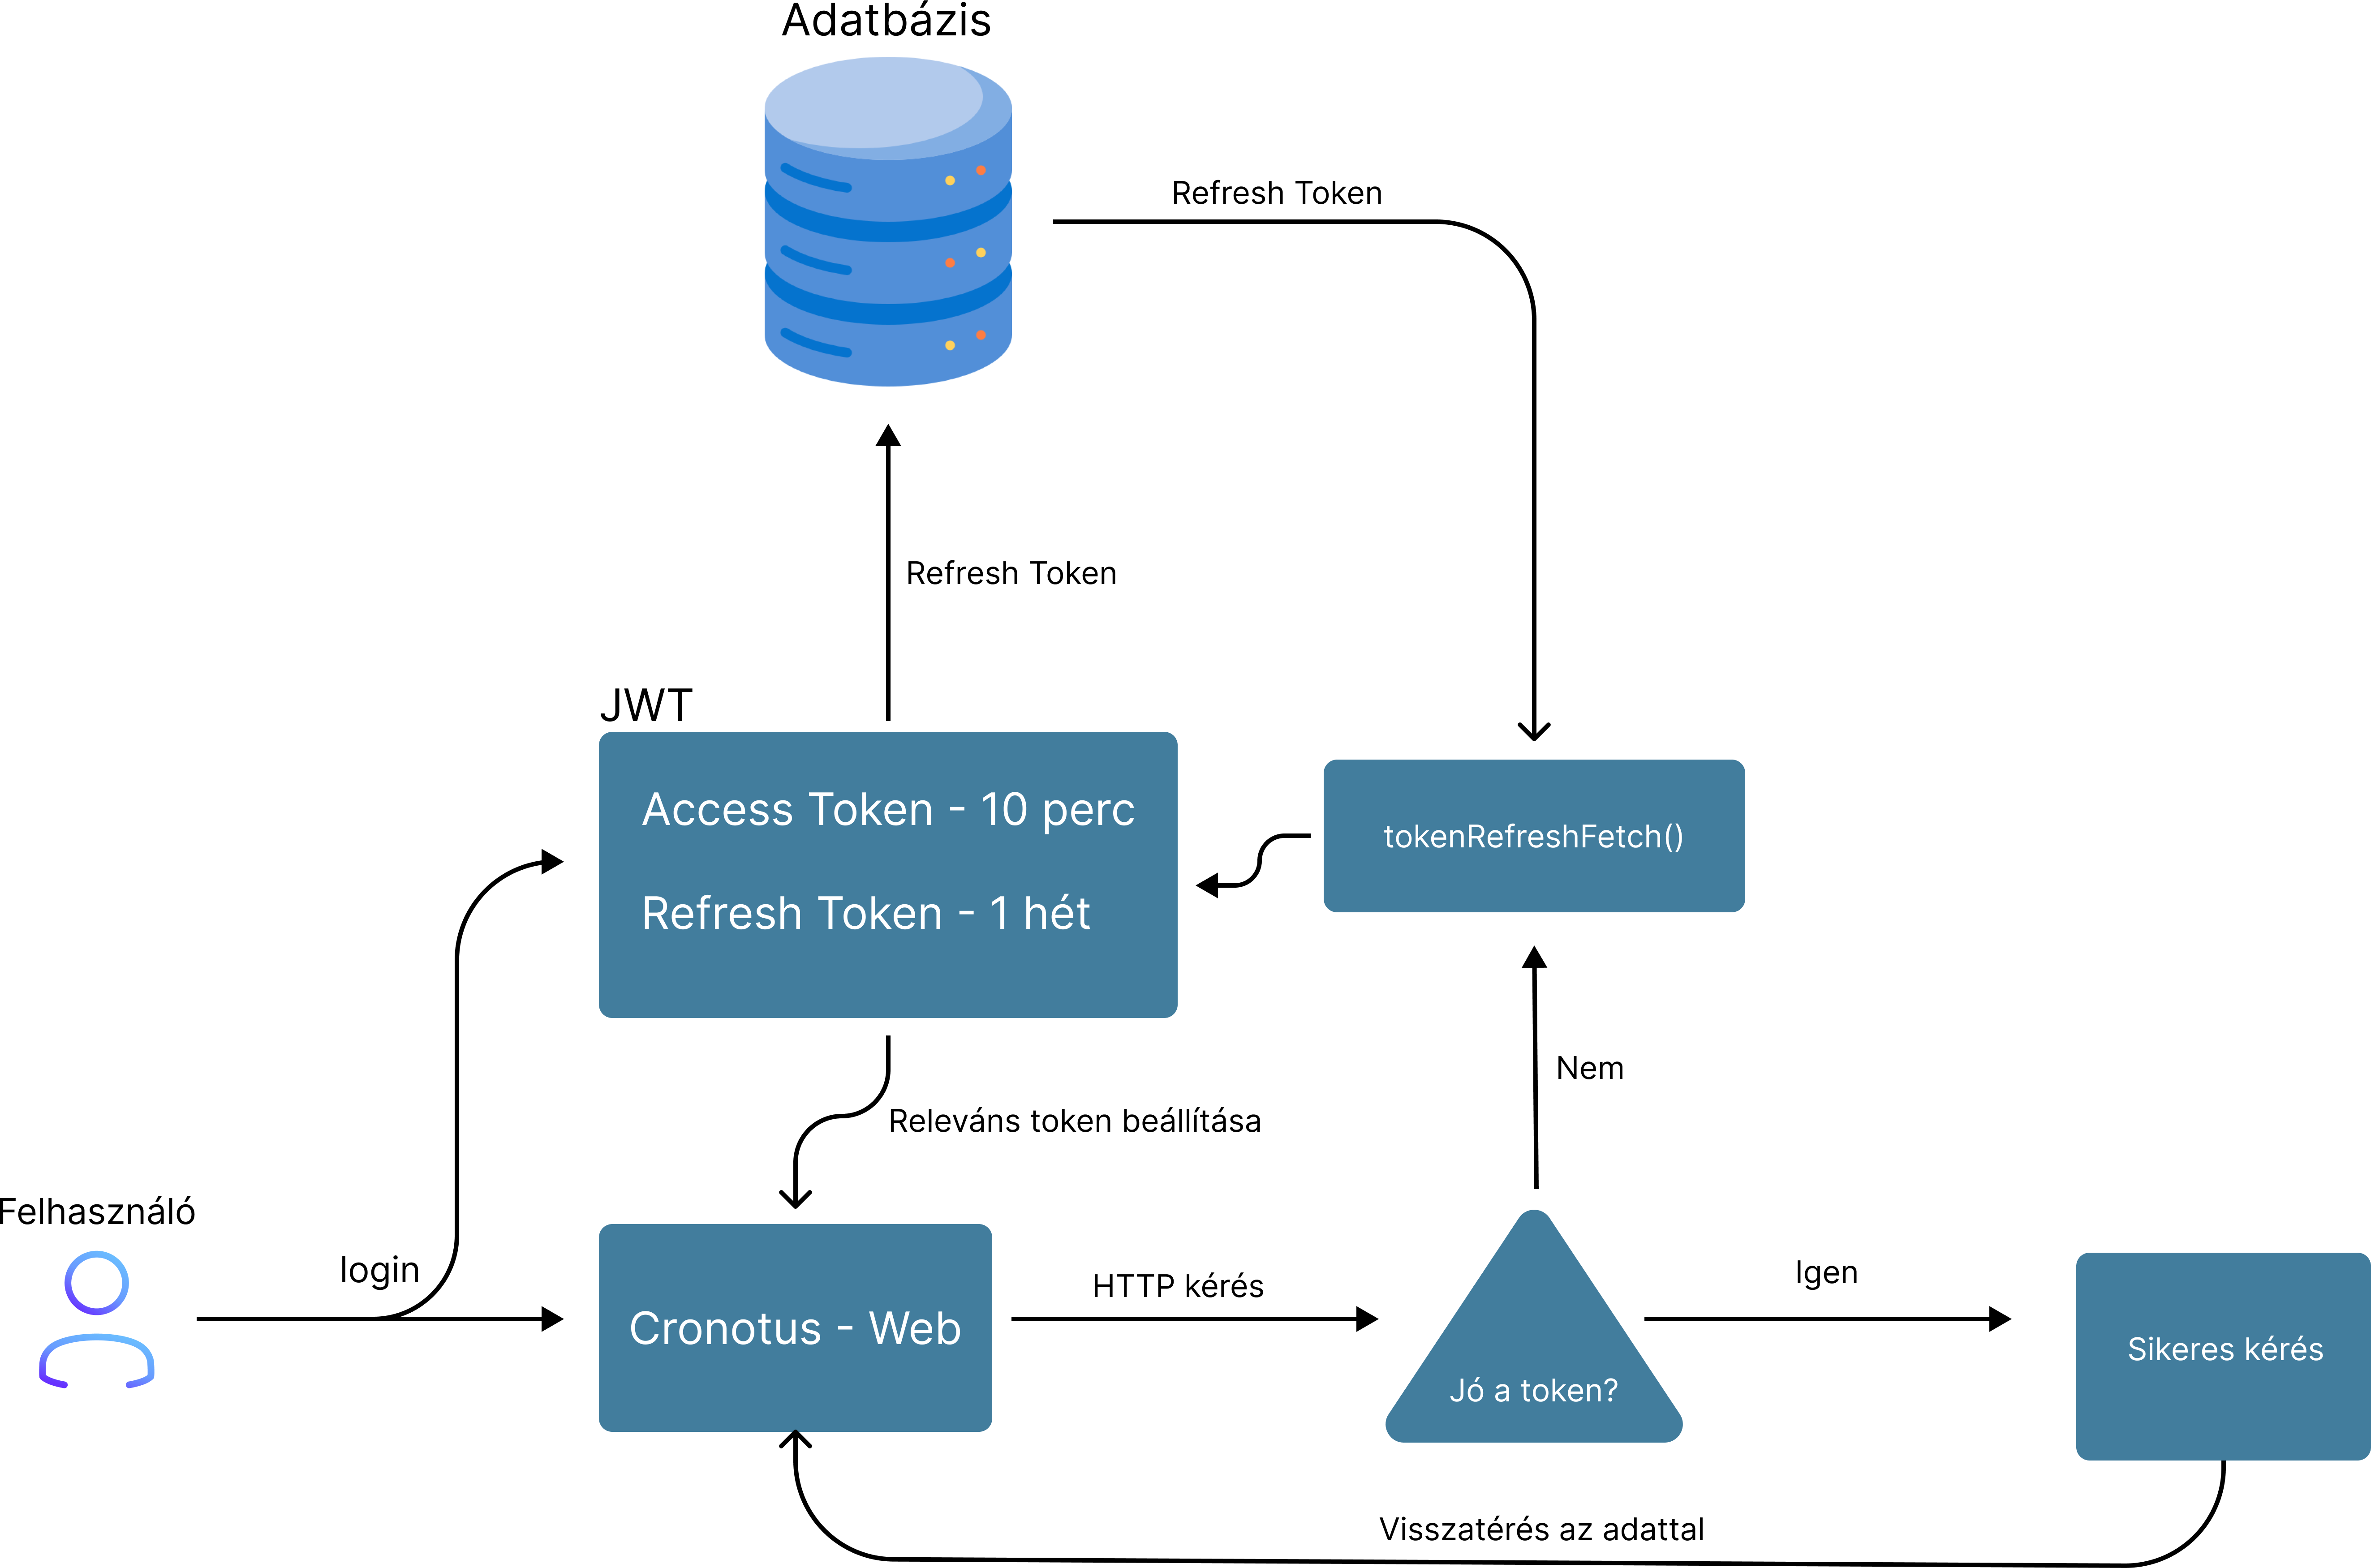
\includegraphics[width=\textwidth]{images/jwt_auth_process.png}
  \caption{A JWT munkamenetkezelés folyamata}
  \label{fig:jwt_auth_process}
\end{figure}
%----------------------------------------------------------------------------

  